%!TEX root = 2024-cmsb_tool.tex
% Take a model from OdeBase or BioModels.
In this section, we show an example workflow using CLUE.
The example described in this section is also available as a Jupyter notebook in \RepoURL.
Suppose we want to study the signaling mechanism in apoptosis as described by kinetic model in~\cite{legewie_mathematical_2006}.

\textbf{Step 1. Model Retrieval.}
To access the required model from ODEBase, we use the following line
\begin{minted}{python}
    model = ode_scrapper(name="BIOMD0000000102")
\end{minted}

\textbf{Step 2. Model Validation.}
Having retrieved the model, we can examine various attributes such as name, size, species, parameters, and equations:
\begin{minted}{python}
    >>> print(model.name)  # Outputs the name of the model
    >>> print(model.size)  # Outputs the size of the model
    >>> print(model.species)  # Lists the biological species
    >>> print(model.parameters)  # Displays the model parameters 
    >>> print(model.equations)  # Shows the model equations
\end{minted}
We get that the original model size is 13.

\textbf{Step 3. Analyses and lumping.}
Following the original paper~\cite{legewie_mathematical_2006}, we are interested in studying the evolution of the observable $C_3$, which is represented as the variable $x7$ in the model.
We first use exact lumping.
To get an exact lumping that preserves $x7$, we use the following line:
\begin{minted}{python}
   >>> exact_lump = model.lumping(['x7'])
\end{minted}
We get a lumped system with a warning that informs us that the size of the lumped system is 13.
TODO:show warning
This means that it was impossible to find an exact reduction.

We can use the approximate lumping functionality of CLUE to increase the aggregation power. 
To this aim, we use the following command 
\begin{minted}{python}
    >>> app_lump_1 = model.app_lumping(['x7'])
\end{minted}
This command relaxes the conditions of exact lumping until it finds a reduction that is smaller than the exact one. 
In this case, the resulting reduction is of size $12$. 

In case we would like to find more significant reductions, it is possible to add a size limit to the approximate lumping with the following command.
\begin{minted}{python}
    >>> app_lump_2 = model.app_lumping(['x7'], max_size=10)
\end{minted}
In this case, the output will be the largest reduction possible having at most 10 lumped species.
The resulting lumped model in this case is of size 7.

\textbf{Step 4. Simulating and comparing models.}
To evaluate the effectiveness of the lumpings, we can simulate the original model and its reductions with the initial conditions and time horizons given in the paper. 
\begin{minted}{python}
    >>> exact_sim = model.simulate(0, 5000)
    >>> app_sim_1 = app_lump_1.simulate(0, 5000)
    >>> app_sim_1 = app_lump_2.simulate(0, 5000)
\end{minted}
We now merge all simulations into one. 
\begin{minted}{python}
   >>> merged_aux = merge_simulations(exact_sim, app_sim_1) 
   >>> merged = merge_simulations(merged_aux, app_sim_2) 
\end{minted}
\textbf{Step 5. Visualizing the results.}
To visualize the results of all three reductions, we use the following line.
\begin{minted}{python}
   >>> create_figure(comp_results, title=['Exact', 'App_12', 'App_7']) 
\end{minted}
The resulting figure is 
\begin{figure}
    \centering
    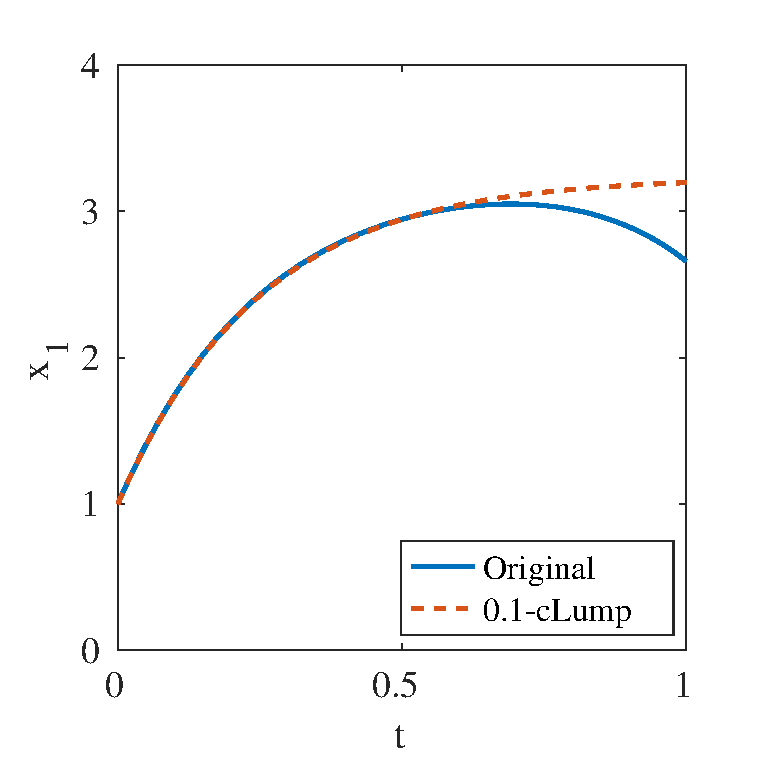
\includegraphics[width=0.3\textwidth]{img/examplecalc.pdf}
    \caption{\comalex{this is a placeholder}
        Time evolution of the $C_3$ concentration using approximate constrained lumping.}
\end{figure}

Add complete code to appendix
Say that we highlight the main commands and the full code listing is in the appendix
Following the approach of the previous cmsb for max\_size


%We begin by getting a model from OdeBase:\\
%\mintinline{python}{)}\\
%To validate the model, we can check its validity via \texttt{model.[attribute]}, where \texttt{attribute} can be the \texttt{name}, \texttt{species}, \texttt{parameters} and \texttt{equations} among others.
%Suppose, we want to study the evolution of the observable $C_3$, this corresponds to the variable $x7$ in the model.
%To construct an exact lumping that perserves the evolution of $x7$ it suffices to use the following line. \\
%\mintinline{python}{exact_lumping = model.lumping([obs_poly])}\\
%\ToolName warns us that the exact lumping found is not a reduction as it has the same size as the original one.

%We can use \ToolName to obtain the next reduction, using the following command \\
%\mintinline{python}{app_lumping = model.app_lumping([obs_poly])}\\
%This command outputs the numerical lumping closest to the exact one.
%Different approximate lumpings can be obtained by providing a value to the \texttt{lumpingTol} keyword argument.
%Similarly, we can explore the attributes of the lumped system.
%For example, we have that \\
%\mintinline{python}{app_lumping.size}\\
%Outputs a reduction of size $12$.
%This is not a significant reduction.
%To ensure we get a small enough reduction we can use the following command \\
%\mintinline{python}{app_lumping = model.app_lumping([obs_poly], max_size=10)}\\
%which will output a reduction with a maximum size of $10$.
%In this case the computed reduction has a size of $7$.

%To see the performance of the approximate lumping we simulate both the original system from 0 to $5000~$seconds using the following lines \\
%\mintinline{python}{exact_sim = model.simulate(0, 5000)}\\
%A similar line outputs the results for the approximate lumped model.
%The simulations can then be merged using \\
%\mintinline{python}{comp_results = merge_simulations(exact_sim, app_sim)}\\
%The merged simulation can be immediately plotted by \\
%\mintinline{python}{create_figure(comp_results, title=['Original', 'Approximate'])}\\
%The resulting plot is show as follows






